\documentclass[UTF8]{ctexart}
	\title{泛做表格}
	\author{唐适之}
	\date{}
	\newcommand{\myparagraph}[1]{\paragraph{#1}\mbox{}\\}
	\usepackage[top=1in, bottom=1in, left=1.25in, right=1.25in]{geometry}
	\usepackage{enumitem}
	\usepackage{graphicx}
	\usepackage{amsmath}
	\usepackage[amsmath,thref,thmmarks]{ntheorem}
	\theoremstyle{nonumberplain}
	\newtheorem{proof}{\hspace{1em}证明:}

\begin{document}
	
	\maketitle
	
	\tableofcontents
	\vfill
	\newpage
	
	\section{Codeforces 238D - Tape Programming}
	
		\myparagraph{题目大意}
		
			有一个包含数字和‘$<$’、‘$>$’的字符串、一个指针和一个指针移动的方向。一开始指针指向最左端的字符,方向向右。做重复操作直到指针指向串外:
			
			\begin{enumerate}
				\item 如果指针指向一个数字,先输出那个数字,然后将这个数字减一。如果这个数字为0就删除它。随后按原指针移动方向移动。
				\item 如果指针指向‘$<$’或‘$>$’,就将指针移动方向调整为尖角所指方向,按此方向移动指针。如果指针指向的下一个字符也是‘$<$’或‘$>$’,就删除原来的。
			\end{enumerate}
			
			给一个长$n$的串$s$和$q$个询问,每个询问给定$l$和$r$,问把$s$从$l$到$r$的子串提取出来做上述操作后,0、1、2、……、9分别会输出多少次。
		
		\myparagraph{算法讨论}
		
			直接在$s$上多次模拟上述操作,直到$s$为空,记录其操作序列。询问的操作序列必然为此操作序列的连续子序列。对每个字符记录指针每次指向它的时间,对于每个询问$(l,r)$,记在$t1$时刻第$l$个字符被第一次访问,此时第$l$个字符的上一个字符为第$l'$个,第$r$个字符的下一个字符为第$r'$个,记$l'$和$r'$在$t1$时刻后首次被访问的时刻是$t2$。这次查询的答案就是在时刻[t1,t2)间输出的每种数字的个数,因为指针在进入[l,r]前不管做了什么操作对此次询问都是没有影响的。在一开始的模拟中记录前缀和即可得出此答案。 
		
		\myparagraph{时空复杂度}
		
			使用链表在$s$上模拟。为了保证严格$O(n)$,可以在链表上仅对数字开节点,跳过‘$<$’和‘$>$’。因为‘$<$’和‘$>$’处不对答案产生直接贡献,只要维护‘$<$’和‘$>$’前后第一个字符的位置,不影响询问,也不影响当‘$<$’或‘$>$’连续时删除‘$<$’或‘$>$’的操作。因为一段连续的数字只会被访问最多10次,即可保证严格$O(n)$,但实际上没有这样做的必要。用诸如std::vector的结构对每个字符存储指针经过它的时间,可以认为插入时间是$O(1)$的,询问时在其上二分以获得$t2$,如果像上面那样跳过‘$<$’和‘$>$’,每个数字被经过次数不超过10,此二分可认为是$O(1)$的。询问中其它操作都是$O(1)$的,询问共耗时$O(q)$。总时间复杂度$O(n+q)$,空间复杂度$O(n)$。
	
	\section{Codeforces 238E - Meeting Her}
	
		\myparagraph{题目大意}
		
			给一个$n$个点,$m$条边的有向图($n$≤$100$,$m$≤$n(n-1)$),Urpal要从$a$点坐公交去$b$点。有$k$条公交线路($k$≤$100$),每条从$s_i$开往$t_i$,每时每刻都有车发出,司机会选择任意一条最短路走。Urpal可以在任意地点上车、下车,但他只知道自己在哪、自己要去哪和自己在哪辆车上,而不知道这辆车要走什么路线。问最坏情况Urpal要坐几辆车才能到,或根本到不了。
		
		\myparagraph{算法讨论}
		
			对于每个从$s_i$到$t_i$的最短路径图,只有在其割点才能确保坐到车。用任意最短路算法求之。设状态$f(x,y)$表示当前到了点$x$,正坐着$y$路车,显然有
			
			$$f(x,y)=\max\left\{\begin{array}{lr}
				f(p,y) & p\mbox{为y的最短路图上x能到达的下一个点} \\
				f(x,q)+1 & q\mbox{为有割点在x的线路}
				\end{array}\right.$$
			
			初始状态为$f(b,...)$,用狄杰斯特拉转移,但不用使用堆。因为转移中权值的变化只有$+0$和$+1$两种,使用一个双向队列,$+0$在前面插入,$+1$则在后面插入即可。
		
		\myparagraph{时空复杂度}
		
			求最短路径图可用弗洛伊德,再用线性算法得到割点,时间复杂度$O(n^3)$。DP状态$O(nk)$,用优化的狄杰斯特拉转移时间$O(n)$,共$O(n^2k)$。总时间复杂度$O(n^3+n^2k)$。空间用在弗洛伊德的邻接矩阵($O(n^2)$)和DP的状态数组($O(nk)$),总空间复杂度$O(n^2+nk)$。可用C++的std::bitset(位运算)在弗洛伊德的同时求出割点,这样算法更简单,但使总时间复杂度上升到$O(n^4+n^2k)$,但$n^4$的常数只有$1/32$,这样的算法也能被接受。
	
	\section{Codeforces 241B - Friends}
	
		\myparagraph{题目大意}
		
			给$n$个数($n \leq 50000$,每个数$\leq 10^9$),要求在其中选出$m$对数(一个数可同时在超过一对中,但两对不能完全相同),使每对两个数的异或之和最大。
		
		\myparagraph{算法讨论}
		
			假设要处理的数在集合$A$中,最高位为第$k$位,此位为0的在子集$B$中,为1的在子集$C$中。那么显然应优先将$B$中的数和$C$中的数配对。若$|B|\cdot|C|\leq m$,那么将它们完全配对,枚举每一位,统计$A$中和$B$中有多少数在此位为1、有多少为0即可计算对答案的贡献。对于剩下的$m-|B|\cdot|C|$次配对机会,将问题转化为关于集合$B$和$C$内部的子问题。否则,$|B|\cdot|C|>m$,仍要分两种情况讨论:记$B$中的数在$k-1$位为0的在子集$D$中,为1的在子集$E$中;$C$中的数在$k-1$位为0的在子集$F$中,为1的在子集$G$中,那么应优先配对$E$和$F$、$D$和$G$。若$|E|\cdot|F|+|D|\cdot|G|\leq m$,将它们完全配对,向上面一样计算贡献,问题转化为关于$D$和$E$配对、$F$和$G$配对的子问题。否则将问题直接转换成关于$E$和$F$配对、$D$和$G$配对的子问题。
			
			以上的问题和子问题都可以表示成$f({X_1,Y_1},{X_2,Y_2},\cdots)$的形式,表示$X_1$和$Y_1$优先配对、$X_2$和$Y_2$优先配对等。可以用队列处理子问题的迭代。
		
		\myparagraph{时空复杂度}
		
			记数的位数为$l$。在所有的问题和子问题中$\{\mbox{集合}1,\mbox{集合}2\}$对的个数为$O(nl)$,因为我们要枚举$l$位,这些集合不会有交,每个问题最多$n$对集合,所以共有最多$nl$对。一开始对读入的数排序,处理每个问题时二分确定某位为0或为1的究竟是哪些数,需要时间$O(nl\log_2n)$。统计对答案的贡献时,每个数仅被扫描一次,每次需枚举每一位,时间$O(nl)$。综上总时间复杂度$O(nl\log_2n)$。计算时要存储读入的$n$个数,并对每个问题存储其$O(n)$个集合对(每个集合在排好序的数组中对应一个连续区间),总空间复杂度$O(n)$。
	
	\section{Codeforces 243D - Cubes}
	
		\myparagraph{题目大意}
		
			有一个水平的正方形,划成$n$×$n$个小格子,每个边长1。这个大正方形作为底面,每个格子向上堆了若干个立方体,立方体棱长1。现在从无限远处以水平方向$(u,v)$观察这个几何结构,问有多少个立方体能被观察到。$n \leq 1000, \mbox{每个格子上的立方体数} \leq 10^9$。
		
		\myparagraph{算法讨论}
		
			记原水平面上的坐标系为$y-x$,为了方便,建新坐标系$y'-x'$,令观察方向为$x'$轴正方向。经过简单的运算可得$x'=xu+yv, y'=yu-xv$(为了保持整数运算,坐标放大$u^2+v^2$倍),对所有小格子都作此变换。把这些格子按观察方向,即$x'$排序,按此方向扫描每个格子,判断该格子上方的立方体有多少被之前扫描的挡住了,把未挡住的统计进答案。为了做到这点,对$y'$坐标离散化,在其上上维护一棵线段树,树上每个区间$[l,r]$表示在$l \leq y' \leq r$上的立方体最矮已经堆了多高。每次有新的格子加入时,先在线段树中查询对应区间中高度的最小值,得出它被挡住了多少,再用此格子的高度更新线段树。
		
		\myparagraph{时空复杂度}
		
			初始化时,需对最多$n^2$个坐标进行排序和离散化,时间$O(n^2\log_2n)$。随后有$n^2$个格子要依次处理,每次需在线段树上询问和插入。总时间复杂度$O(n^2\log_2n)$。总空间复杂度$O(n^2)$。
	
	\section{Codeforces 254D - Rats}
	
		\myparagraph{题目大意}
		
			有一个$n$×$m$的网格($n,m \leq 1000$),每个格子要么是空的,要么是墙,要么是老鼠。你要引爆两颗手榴弹,所有与任一手榴弹距离不超过$d$($d \leq 8$)的老鼠都会被清除。这里的距离指的是连接手榴弹和老鼠的不经过墙的最短四连通路径的长度。求出一对合法的手榴弹位置,或输出无解。
		
		\myparagraph{算法讨论}
		
			$d \leq 8$是突破口。对于任意一只老鼠,肯定有一个手榴弹要在与它距离不超过$d$的地方引爆,随便选一只老鼠,做深度最深为$d$的BFS,找出所有可能位置。枚举这$O(d^2)$个位置作为其中一个手榴弹的引爆点,做深度限制为$d$的BFS找出被其清除掉的老鼠。接着,找出还活着的随便一只老鼠,这一步可以通过将老鼠储存在std::set之类的容器中快速完成。第二颗手榴弹的引爆点与这只老鼠的距离也不能超过$d$,理由同上。以这只老鼠为中心做类似的BFS,找出第二颗手榴弹可能的$O(d^2)$个引爆位置,枚举这个位置,再用一个类似的BFS检查是否所有老鼠都被清除。
		
		\myparagraph{时空复杂度}
		
			枚举第一颗手榴弹的位置耗时$O(d^2)$,每枚举一次需:(1)用$O(d^2)$时间清除一部分老鼠;(2)用$O(d^2)$枚举第二颗手榴弹的位置,每次再$O(d^2)$确认是否老鼠都被清除。共耗时$O(d^6)$,加上读入的时间$O(n^2)$,总时间复杂度$O(n^2+d^6)$。总空间复杂度$O(n^2)$。
	
	\section{Codeforces 256D - Liars and Serge}
	
		\myparagraph{题目大意}
		
			有$n$个人,有人说真话有人说谎。现在问他们每个人有多少人在说真话,他们每人给出了自己的答案$a_i$。给定$n$、$k$,问有多少种${a_i}$可以判断出至少有$k$人在说谎。$1 \leq k \leq n \leq 2^8$。保证$n$是2的整数次幂。
		
		\myparagraph{算法讨论}
		
			判断出一些人在说谎当且仅当他们说出的数字和说这个数字的人的数量不相等。用DP解决。从小到大处理说每个数字的人,设$f[i][j][k]$表示当前处理到数字$i$,已经处理了$j$个人,其中有$k$人被确定是说谎者,易得转移方程:
			
			$$f[i][j][k]=\sum_{p=0}^k f[i-1][j-p][k-p] \cdot \binom{j}{p} (p\not=i) + f[i-1][j-i][k]$$
			
			这个DP是$O(n^2k^2)$的,无法通过。但是$n$为2的整数次幂,只能取9个值。可以打表通过。
		
		\myparagraph{时空复杂度}
		
			打表。打表时间$O(n^2k^2)$,实际时间$O(1)$。打表所需空间$O(n^2k)$,实际所需空间$O(n^2k)$。
	
	\section{Codeforces 264E - Roadside Trees}
	
		\myparagraph{题目大意}
		
			在一条直线有n个位置可以种树($n \leq 10^5$),自西向东标号1至n。每个月,每棵树都会长高1米。每个月初有一个操作,操作有两种类型:
			
			\begin{enumerate}
				\item 在位置p种一棵高度为h的树。($1 \leq p \leq n, 1 \leq h \leq 10$)
				\item 砍掉从西向东数的第x棵树,当这个位置的树被砍掉后,这个位置不能再种树。($1 \leq x \leq 10$)。
			\end{enumerate}
			
			每次操作后输出树高的最长上升子序列长度。
		
		\myparagraph{算法讨论}
		
			回顾用数据结构做${a_i}$的最长上升子序列的方法:做到第$i$个数时,在数据结构中查询$i$之前最大的一个小于$a_i$的数是多少,用它更新最长上升子序列,插入数据结构。类似的,我们也可以扫描数列元素的值,从大到小做到值为$i$的数时,在数据结构中查询坐标大于该数坐标的最小一个坐标,用它更新最长上升子序列,插入数据结构。这两种方法本质是一样的。这里我们要结合这两种方法。
			
			同时维护上述的两个数据结构。当新种树时,一定是树高最小的10棵之一,暴力在数据结构中撤销这最小的10个,然后按上面的第二种方法重新计算,更新这种方法对应的数据结构时同时更新另一种方法的数据结构。当要砍树时,砍的树一定是最西边的10棵树之一,类似的,暴力撤销这10棵,然后重新计算。撤销时每次在数据结构中找最小(或最西)即可找到这十个,也可以另维护堆或set。
		
		\myparagraph{时空复杂度}
		
			数据结构可用线段树实现,每次种树或砍树时间复杂度$O(\log_2n)$,总时间$O(n\log_2n)$,有常数10。空间复杂度$O(n)$。
	
	\section{Codeforces 269E - String Theory}
	
		\myparagraph{题目大意}
			
			给一个矩形,两条竖边上分别均匀分布N个点,两条横边上分别均匀分布M个点(N,M≤$10^5$),每个点向另一个不在同一边上的点连了一条线。输出一个重排行和列的方案使这些线不相交,或输出无解。
			
		\myparagraph{算法讨论}
		
			构造出解。从一个点出发,交替地先走到与该点相连的点上,再走到与第二个点有公共行/列的点上,直到走回初始点,这样的路径称为\emph{环}。如果两条线都连接着矩形的相同两条边,那么认为这两条线的方向是相同的。如果从一个环的任意节点按任意方向出发所经的线,与从另一个环的任意节点按任意方向出发所经的线对应方向相同,则认为这两个环是相同的。注意到无论如何变换行和列的顺序,环都相同;如果两个矩形中的环都相同,其中一个矩形也一定可以通过重排行和列变换到另一个矩形。样例的环如下图用不同颜色表示:
			
			\begin{figure}[ht]
				\centering
				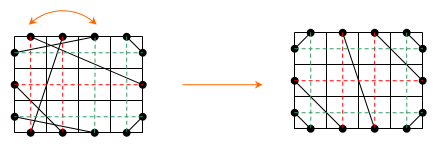
\includegraphics[width=\textwidth]{fig269e_1.jpg}
				\caption{环}
			\end{figure}
			
			有一类环只包括一条上到右的线、一条右到下的线、一条下到左的线和一条左到上的线,把这类环顺次排列到矩形的四角,设这样的环有A个。不妨考虑矩形的横边长于竖边,设有B条从上到下的线(注意不会有从左到右的线,事实上A=M-N),合法解中要么还有M-2A-B条线从上连到左、有M-2A-B条线从右连到下,要么还有M-2A-B条线从上连到右、有M-2A-B条线从左连到下(这些线不在那4A条线中),此外就没有别的线了。这2(M-2A-B)条线中,每一对有端点在同一行的,记为一组,这一组可以表示为一条从上到下的路径(注意到所有这些线都成组,每组两条线一条连接着上边,一条连接这下边),此外那B条从上到下的线也可以分别表示一条路径。这些路径的上下端点都分布在A+1$\sim$M-A列上,可以将这些列提取出来,标号为0$\sim$M-2A-1。观察到这些路径是平行的,对于上端点标号i的,下端点一定标号(i+k) mod (M-2A),k是一个整数。这样这些路径就可以写成一个列编号的轮换:
			
			$$\begin{pmatrix} 0 & 1 & ... & M-2A-1 \\ k & k+1 & ... & k-1 \end{pmatrix}$$
			
			仅由一条从上到下的线构成的路径\textbf{连续}地分布在矩形的中间,另外的由两条线构成的路径分布在两侧,所以这些路径构成了$\frac{M-2A-1}{gcd(M-2A-1,k)}$个\textbf{相同}的环,只要知道M,A,B,每个环都是已知的,依次将读入矩形中的环对应移动至这些环中即可。
		
		\myparagraph{时空复杂度}
		
			首先我们需要找出读入数据中的环,这一步是线性的。然后要找出一类环移动到矩形的四角,这一步也是线性的。对于剩下的环,用合法解的环建一个KMP,再用二倍长度的读入数据中的环匹配判断是否相同(循环同构),如果是则将其移动至对应位置,这一步也是线性的。如果以上任意一步失败则输出无解。整个过程是线性的,时间复杂度$O(N+M)$,空间复杂度$O(N+M)$。
	
	\section{Codeforces 274E - Mirror Room}
		
		\myparagraph{题目大意}
			
			给一个n×m的网格,有k个格子是镜子(1≤n,m≤$10^5$,0≤k≤$10^5$)。光从一点发出,遇到镜子会像下图一样反射:
			
			\begin{figure}[ht]
				\centering
				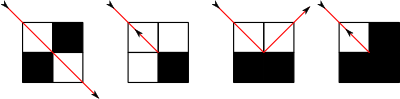
\includegraphics[width=\textwidth]{fig274e_1.png}
				\caption{反射}
			\end{figure}
			
			求光路会经过多少个格子,重复经过不计。
			
		\myparagraph{算法讨论}
		
			一个可行的方案是直接用复杂的数据结构模拟,直到光路进入循环,但是题目中的一些性质可以使解法更简单。首先显然光会以原方向回到起点才进入循环,其次光不会以交叉的方向通过同一个格子两次,这点对格子黑白染色后就能发现,这样就省去了判重的步骤。先处理出每个反射点,对每条对角线都建一个数据结构(C++可用set,也可以不建数据结构而使用二分),插入反射点。直接进行模拟,每次可在数据结构上找出光的下一个反射点的位置以及反射后的方向,对光路上的每条线段累加其长度即可,直到回到起点。对于中途“掉头”的光路,可分起点前和起点后两部分分别计算。
		
		\myparagraph{时空复杂度}
		
			我们是统计不重复的光路,光路上的反射点最多$O(n+m+k)$个,数据结构的时间$O(\log_2k)$。总时间复杂度$O((n+m+k)\log_2k)$,空间复杂度$O(n+m+k)$。
	
	\section{Codeforces 280E - Sequence Transformation}
	
		\myparagraph{题目大意}
		
			给一个不递减序列$\{x_i\},(1 \leq i \leq n, 1 \leq x_i \leq q)$,要求把序列转化为新序列$\{y_i\},(1 \leq i \leq n, 1 \leq x_i \leq q)$,并满足$a \leq y_{i+1}-y_i \leq b,(1 \leq i < n)$,转化代价为$\sum_{i=1}^n(y_i-x_i)^2$。找出使代价最小的$\{y_i\}$。($1 \leq a,b,q \leq 10^9, 1 \leq n \leq 300000$,数据比CF原题的大)
		
		\myparagraph{算法讨论}
			
			记$y_i=v$时的代价函数为$f_i(v)$,假设$f_i$是一个先递减后递增的函数,记其最小值点为$v=min$,设
			
			$$\begin{aligned}
				g_i(v)&=\min_{v-B \leq v' \leq v-A}f_i(v')\\
				      &=\begin{cases}
				           f_i(v-A) & v < min+A \\
						   f_i(min) & min+A \leq v < min+B \\
						   f_i(v-B) & v \leq min+B
						\end{cases} \\
				f_{i+1}(v)&=\min_{v-B \leq v' \leq v-A}f_i(v')+(v-x_{i+1})^2 \\
				          &=g_i(v)+(v-x_{i+1})^2
			\end{aligned}$$
			
			显然$f_1(v)=(v-x_1)^2$是一条开口向上的抛物线,是先递减后递增的函数。$f_i$每次变换为$g_i$后显然还是先递减后递增的函数,再加上$(v-x_{i+1})^2$后,因为两个导数递增的函数相加依然导数递增,$f_{i+1}$依然保持此性质,故上述转移可行。
			
			每次转移我们需要的操作是 1.查找一个先递减后递增函数的最小值 2. 将函数的一部分左右平移。 3. 在函数中插入一段。 4. 将函数整体加上一个二次函数。 因为$f_i$的每一段都是一个二次函数的一部分,可用一个平衡树维护其每一段,并执行上述操作,以此做到快速转移。最后查找$f_n$的最小值即最优解。记录下每一次转移的$min$值,即可由最后的最小值逆推回每个$y_i$。
			
		\myparagraph{时空复杂度}
		
			$O(n)$次转移,每次耗时$O(\log_2n)$,总时间复杂度$O(n\log_2n)$。每次转移在函数中最多新增一段,空间复杂度$O(n)$。
	
	\section{Codeforces 286D - Tourist}
	
		\myparagraph{题目大意}
		
			有些时刻会有点$A(1,0)$和$B(-1,0)$同时以1单位每秒的速度向$y$轴正方向移动,而另某些时刻会有墙出现,从$(0,l)$延伸到$(0,r)$。墙瞬间出现,且出现后就不消失,而且多堵墙间可以有重叠。问对于每对$(A,B)$,在其运动过程中有多少秒$AB$连线会与至少一堵墙相交。共$n$对$(A,B)$、$m$堵墙,$n,m \leq 10^5$。
		
		\myparagraph{算法讨论}
		
			建立另一个坐标系$y-t$,$A$和$B$的轨迹在其上对应一条斜率为1的射线,表示在每时刻它们的$y$坐标为多少。对每堵墙作矩形:记其出现时刻为$t$,它的左下角为$(t,l)$,左上角为$(t,r)$,向右无限延伸。这样问题可以转化为$A$和$B$对应的射线与任意矩形相交部分的总长为多少(答案要乘$\frac{\sqrt{2}}{2}$)。
			
			由于墙可能有重叠,要先把它处理成不重叠的以便后续工作。把墙对应的矩形按左边界的$t$坐标从小到大排序,用一个std::set或其他类似数据结构记录其上下边界的$y$坐标。每添加一个新的矩形,查找它与哪些已添加的矩形相交。如果与新添加矩形相交的矩形的$y$坐标区间被新矩形的$y$坐标区间完全包含了,就结束被包含的矩形,即将其右边界设为新矩形的左边界。如果只被部分包含,就缩小新矩形的范围使之不再相交。
			
			现在,为了方便,将坐标系作如下变换:$(t,y) \to (t-y,y)$。这样$(A,B)$对应的射线就平行于$y$轴了,而且答案不再需要乘$\frac{\sqrt{2}}{2}$了。此时原来的矩形变成了梯形,其左边的斜率为-1。再次为了方便,可以将其看成一正一负两个三角形。记该三角形的最左边的顶点坐标为$(p,q)$,若它与$(A,B)$对应的射线(记其为$t=t0$)相交,那么它对答案的贡献为$t-p$,即总答案为:$t$乘以与射线相交的三角形个数,减去与射线相交的三角形的$p$之和。将三角形和射线都按按新坐标系的$t$坐标从小到大排序,从小到大扫描并维护答案即可。
		
		\myparagraph{时空复杂度}
		
			去除墙的重叠需使用set,时间$O(m\log_2m)$。最后的扫描需将墙和射线都排序,时间$O(m\log_2m + n\log_2n)$。总时间复杂度$O(m\log_2m + n\log_2n)$。总空间复杂度$O(n+m)$。
	
	\section{Codeforces 306D - Polygon}
	
		\myparagraph{题目大意}
		
			对于给定$n$($3 \leq n \leq 100$),构造任意一个合法多边形,满足其所有内角相等,任意两个边长的差的绝对值大于等于$10^{-3}$,边长$\in [1,1000]$,横纵坐标的绝对值小于等于$10^6$。
		
		\myparagraph{算法讨论}
		
			首先,直观地看,$n$越大角度相同的限制的影响越小,可以发现$n \leq 4$时是无解的,其它情况都有解。一个很自然的想法就是对多边形的每条边按一个方向(比如逆时针)逐一随机其长度,每条边相对于上一条边旋转一个角度。但这样可能构不成多边形,原因有两种:末边未能与多边形接合、末边不是与起点而是多边形的其它部分接合了。如图:
			
			\begin{figure}[ht]
				\centering
				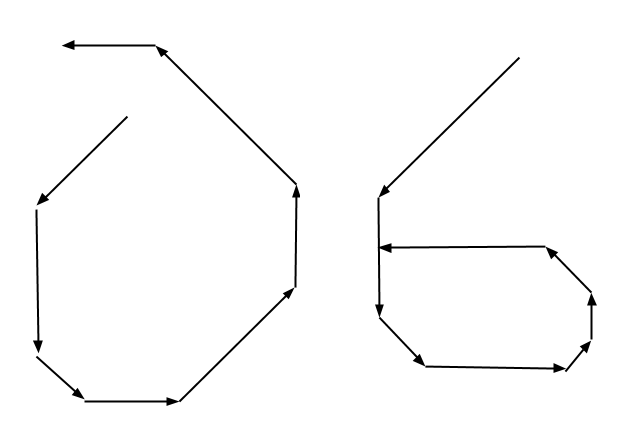
\includegraphics[width=0.6\textwidth]{fig306d_1.png}
				\caption{n=8时两种不能构成多边形的情况}
			\end{figure}
			
			首先对其进行粗略的修正。对于第一种情况,只需限制任何边不得超过初始边所在直线即可。对于第二种情况,对于任意边A,过多边形起点作A的下一条边的平行线,显然A至少要穿过这条平行线才有解。如图:
			
			\begin{figure}[ht]
				\centering
				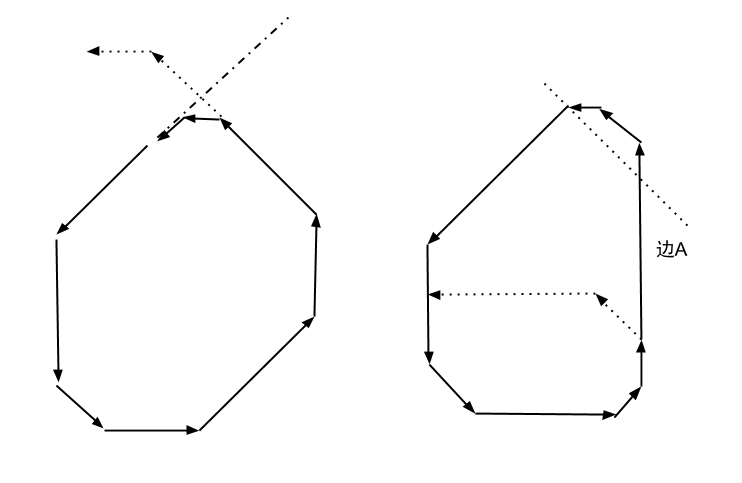
\includegraphics[width=0.6\textwidth]{fig306d_2.png}
				\caption{n=8时两种不能构成多边形的情况}
			\end{figure}
			
			显然这两种限制都只是得出合法解的必要条件,还有一个重要因素是题目中边长的限制。如果仅要求边长大于等于0而不是大于等于1,并且没有边长不相等的限制,则可以看出仅按上述限制是可以构造出解的。在有了边长限制后,就不能使某一条边只是恰好达到了上述限制,还要为后续的边长限制预留空间。需要预留的空间与剩余边数有关,剩余边数越大需要预留的空间越大。这一点比较难计算,但因为读入总共只有98种情况,又可以很轻松地写出检验程序,我们可以调整参数多次尝试。当然,也不能只是把预留空间尽量留大,因为要考虑到边长还有上限1000,而且随机的范围不能太小,以免有两边的长度过于接近。综合以上因素调整参数即可。
		
		\myparagraph{时空复杂度}
		
			实现上,只需依次在一定范围内随机每个边长,每次计算是$O(1)$的,总时间$O(n)$。总空间$O(1)$。
	
	\section{Codeforces 309D - Tennis Rackets}
	
		\myparagraph{题目大意}
		
			有一个等边三角形,每边上有$n$个$n+1$等分点。要在每边上分别选一个点,而且每条边都不能选靠近三角形顶点的$2m$个点,使选出的三个点形成钝角三角形。求方案数。$n \leq 32000$。
		
		\myparagraph{算法讨论}
		
			显然,若已知选出的其中两个点,不管在新三角形中是一个钝角顶点一个锐角顶点,还是两个锐角顶点,都是可以在$O(1)$时间内算出另一个点的,这样可以构造$O(n^2)$算法。不过,这就是时间复杂度最快的方法,所以要进行常数优化。
			
			由于时间复杂度很大,达到了$32000^2$,直接实现的常数也不大,影响常数优化的每个细节都要考虑。并且,有时常数优化不是语句和表达式看起来简短就能使程序快的,要多在自己的机子上尝试,然后找出最快的写法。当然运气好也可以一下子通过,应根据具体语句分析。下面给出若干个需要考虑,但不一定要完全遵循的地方:
			
			\begin{enumerate}
				\item 利用对称性将时间折半。如果枚举的是两个锐角顶点,这两个点离钝角顶点所在边的距离分别为$a$和$b$与分别为$b$和$a$的方案数是相同的。如果枚举的是一个钝角顶点和一个锐角顶点,那么钝角定点距离其所在边一段$a$和$N+1-a$时的方案数是相同的。
				\item 是解方程还是利用单调性维护?枚举出两点$A$和$B$后,$C$的范围可以解方程得出,虽然语句短,但这样需要开平方或者除法。事实上$C$的范围是单调的,可以直接维护一个变量表示,判断时只需乘法和加法,反而更快。
				\item break。因为上述$C$的范围是单调的,制定适当的循环顺序,当$C$范围为空时可break。
				\item 预处理循环范围。与上面相似,可以解方程直接得出循环范围,这样不仅能像break一样提早结束循环,还能推迟循环开始。不过经测试这样提升的速度并不能超过随机误差。
				\item 是枚举两个锐角点还是一个钝角点一个锐角点?经实验后者所需循环次数更少。
				\item 避免复杂的表达式而用变量维护?$C$的范围表达式比较复杂,可以考虑用一个变量维护,每次加上此次与上一次的差。这对时间的贡献应具体情况具体分析。
				\item 一些其他的因素。有时看似更慢的表达式更快,应多次尝试。此外,我发现诸如变量是开局部变量还是全局变量等因素对事件都是有影响的。
				
			\end{enumerate}
		
		\myparagraph{时空复杂度}
		
			时间复杂度$O(n^2)$,空间复杂度$O(1)$。
	
	\section{Codeforces 316G3 - Good Substrings}
		
		\myparagraph{题目大意}
		
			给定一个字符串$s$和$n$个三元组$(p_i,l_i,r_i)$,要求算出满足如下要求的$s$的不同子串的个数(相同子串不计):该子串在每个$p_i$中出现次数在区间$[l_i,r_i]$中。字符串$s$和$p_i$的长度均不超过50000,$0 \leq n \leq 10$。
		
		\myparagraph{算法讨论}
		
			把所有读入的$n+1$个字符串串联起来,中间用未出现过的不同字符隔开,建一个后缀数组。对于$s$的每个后缀$t$,考虑这个后缀有多少个前缀满足要求。假设满足要求的前缀长度为$l$,有多少个来自$p_i$的后缀与$t$的LCP不小于$l$,该前缀就在$p_i$中出现了多少次。因为后缀数组中与$t$的LCP在$rank[t]$两侧是单调的,所以满足要求的$p_i$的后缀都在一个范围内连续分布,所以可以根据$l$二分出此范围。对于每个$i$预处理出一个前缀和,其中的第$j$个元素表示在后缀数组中前$j$个后缀中出现了多少次来自$p_i$的后缀,这样就可以根据上述范围判断$l$是否大了或小了。据此可以二分出$l$的区间。对于每个$t$累加$l$的区间长度即为答案。
		
		\myparagraph{时空复杂度}
		
			记读入的字符串总长为$L$。首先建立后缀数组,使用倍增法的时间为$O(L\log_2L)$。为了在$O(1)$时间内求LCP,还要用$O(L\log_2L)$的时间预处理$height$数组的RMQ。求解时,先二分$l$。对于每个$l$,先$O(\log_2L)$二分出满足要求的后缀范围,再利用前缀和$O(n)$判断是否合法。综上,总时间复杂度为$O(L\log_2L+(\log_2L+n))$。总空间复杂度$O(L\log_2L)$(RMQ)。
	
	\section{Codeforces 317E - Princess and Her Shadow}
	
		\myparagraph{题目大意}
		
			公主在追她的影子。地图是一格一格的,一开始她们在不同的格子里,每次公主可以向上下左右某一方向移动一格,此时影子会模仿她的动作,例如她向右走影子也向右走。但是地图上有些格子有树,公主不能移动过去。如果影子模仿公主时会撞树影子则会放弃这次模仿,但公主仍能移动。有M棵树,M≤400。-100≤树的坐标≤100,但公主和影子可以走出这个范围。给定公主、影子的初始位置和树的位置(读入的坐标都不相同),求一个合法的方案使公主追上影子,或输出无解。
		
		\myparagraph{算法讨论}
			
			如果公主的位置和影子的位置不连通,则无解。如果没有任何一棵树,显然也无解。否则一定有解。
			
			如果公主可以移动出[-100,100]的坐标范围,影子也能移动出去,就先让她们移动出去。如果公主的纵坐标比影子更大,就控制影子走到最上面一棵树上方,公主向下走;如果公主的纵坐标比影子更小,就控制影子走到最下面一棵树下方,公主向上走。用类似的方法调整横坐标,即可追上影子。
			
			如果公主走不出[-100,100]的范围,找一条合法的移动序列从公主的初始位置走向影子的初始位置。公主依照这个序列走,每次影子移动了,就把影子的移动方式加到序列的尾部,相当于公主在跟着影子。因为公主走不出[-100,100]的范围,影子也走不出,公主每走200步影子至少被卡住一次,否则影子就走出这个范围了,若影子被卡住了,公主和影子的距离便减小,否则她们的距离不变,最终公主能追上影子。
			
		\myparagraph{时空复杂度}
			
			如果公主和影子可以移动出[-100,100]的坐标范围,最多100×100的广搜就能使她们移动出去,后面每一次调整不超过5×100步,总步数不超过105×100步。如果她们不能移动出去,她们的初始距离最多100×100(这里的距离指的是不穿过树走过去的路程),最多每200步此距离就会减少一次,步数上限是100×100×200。显然执行每一步是$O(1)$的,总时间最大100×100×200,空间100×100。
	
	\section{Codeforces 325D - Reclamation}
		
		\myparagraph{题目大意}
		
			有一个r×c的地图,把左边界和右边界粘起来使得形成一个圆柱,现在要不断地请求挖去其中的格子,共k次请求,要求任何时候都存在一条从最上方到最下方的路径(四联通),如果某次操作不满足要求则不做,问最后有多少次操作是成功的。
		
		\myparagraph{算法讨论}
		
			把判断上下的格子是否连通,转化为判断是否存在一条由挖去的格子组成的八连通路径,环绕整个圆柱。每次挖去新格子时就要判断是否形成了这样一条路径。用如下方法判断:将地图复制一遍拼接在右侧,再左右相接,即形成一个r×2c的地图。原来挖去的格子(x,y)现在对应两个格子(x,y)和(x,y+c)。存在上述路径等价于存在一条路径从(x,y)连接到(x,y+c)。
			
			\begin{proof}\mbox{}\\
			
				若从(x,y)向右走能到(x,y+c),地图左右两半一样,从(x,y+c)继续向右走越过边界也能到(x,y),即存在环绕圆柱的路径;若存在环绕圆柱的路径,从路径上的任一格子(x',y')必然能走到(x',y'+c),而挖去(x,y)前并不存在这样的路径,若挖去(x,y)就能存在,必然有(x,y)与(x,y+c)连通。
			
			\end{proof}
		
		\myparagraph{时空复杂度}
		
			用并查集做上述操作,(x,y)与(x,y+c)连通即它们在同一个并查集中。每次要挖去新格子时扫描与其相邻的格子即可判断,若合法就将新格子和与它相邻的格子合并。每次判断或合并都是$O(1)$的,时间复杂度共$O(k)$。空间复杂度$O(rc)$。
	
	\section{Codeforces 331E2 - Deja Vu}
		
		\myparagraph{题目大意}
		
			给一个n个点,m条边的有向图(n≤50,m≤$\frac{n(n-1)}{2}$),每条边上有一个序列。对于每个1≤l≤2n,统计图上有多少个长度为l的路径,满足其依次经过的点组成的序列等于其依次经过的边上的序列的顺次拼接。
			
		\myparagraph{算法讨论}
		
			构造出解。定义元路径,任何合法路径可以表示为若干以下三种元路径的拼接,这三种元路径的任意子路径都不是元路径:
			
			\begin{enumerate}
				\item 满足其本身就是合法路径的。
				\item 满足其边上序列拼接成的序列在左端添加路径的起始节点后,就和依次经过的点组成的序列相同的。
				\item 满足其边上序列拼接成的序列在右端添加路径的终末节点后,就和依次经过的点组成的序列相同的。
			\end{enumerate}
			
			我们定义扩展操作为,选择一条路径,迭代地将这条路径扩展为,这条路径依次经过的边上的序列拼接构成的序列对应的路径,直到该路径成为一个合法的元路径为止。可以证明任何元路径都可以由某条边经过扩展操作得到,三种元路径的证明依次如下:
			
			\begin{enumerate}
				\item 第一种元路径中一定含某条边x$\rightarrow$y满足此边的序列中包含相邻的x,y,用这条边可以拓展出这条元路径。证明:路径的节点数比边数大1,由鸽笼原理得路径中必然有至少一条边p$\rightarrow$q的序列包含至少两个元素,如果它不包含相邻的p,q,就用这条边把路径割开,其中一侧肯定边数比边的序列中元素数小,递归下去一定能找到这样一条x$\rightarrow$y。因为x$\rightarrow$y的序列中包含相邻的x,y,所以无论怎么扩展x$\rightarrow$y都在路径中,必然能扩展出元路径。
				\item 第二种元路径可以用其起始边扩展出。设这条边为x$\rightarrow$y,其序列的起始元素一定是y,无论怎么扩展x$\rightarrow$y都在路径中,必然能扩展出元路径。
				\item 第三种元路径可以用其终末边扩展出。设这条边为x$\rightarrow$y,其序列的结尾元素一定是x,无论怎么扩展x$\rightarrow$y都在路径中,必然能扩展出元路径。
			\end{enumerate}
			
			处理出元路径后,DP算出答案。首先定义单位路径为,第一种元路径后面可连接第二种元路径而前面可连接第一种元路径形成的路径。显然单位路径是合法路径,而且所有合法路径一定由一条或多条单位路径通过序列为空的边连接而成。设f[i][j][k]表示从j到k有一条长度为i的单位路径的条数,可枚举元路径转移。设t[i][j][k]表示j到k长度为i的,先经过一条序列为空的边,再经过一条单位路径的合法路径条数,可用f得到t。设g[i][j]表示长度为i,结束于j的合法路径条数,可用t获得g。对每个i统计g[i][j]的和即为答案。
		
		\myparagraph{时空复杂度}
		
			最多有$O(n^2)$条边要扩展,单次扩展操作时间$O(n^2)$,扩展共耗时$O(n^4)$,由此也可知元路径和单位路径的总数都是$O(n^2)$的。从元路径获得f需$O(n^4)$,从f获得t需$O(n^4)$,从t获得g需$O(n^4)$,总时间复杂度$O(n^4)$。空间复杂度为DP数组空间复杂度,为$O(n^3)$。
	
	\section{Codeforces 335E - Counting Skyscrapers}
	
		\myparagraph{题目大意}
		
			有一列摩天楼,楼的个数在正整数集上均匀随机,每一栋楼高$h$的概率分别都是$2^{-h}$($h>0$),每栋楼的高度相互独立。一栋高$h$的楼楼层从0到$h-1$编号。假设两栋楼都有第$i$层,且两栋楼间所有楼的最高层都小于$i$,那么这两栋楼的第$i$层就会连接一条空中走廊,两栋楼间可能有多条空中走廊。Alice数了楼的准确数量$n_{Alice}$,Bob采取如下方法估计楼的数量$n_{Bob}$:他从第一栋楼开始走,此时计数器设为1,每次尽量用最高的但不高于第$H$层的空中走廊向前走($H$给定),若该走廊在第$i$层则计数器增加$2^i$,最后计数器的数字便是$n_{Bob}$。任务是用$n_{Alice}$求出$n_{Bob}$的期望值或用$n_{Bob}$求出$n_{Alice}$的期望值。
		
		\myparagraph{算法讨论}
			
			若给定$n_{Bob}$,$E(n_{Alice})=n_{Bob}$。(注:以下部分pdf阅读器偶尔不能正确加载某些字符,如出现此情况,重新打开即可)
			
			\begin{proof}\mbox{}\\
			
				对于Bob走的每条空中走廊,假设它高$h$,其下方每栋楼的高度(最高层+1)都要小于等于$h$,概率为$1-\frac{1}{2^h}$。走廊不短于$L$的概率为$(1-\frac{1}{2^h})^L$。则走廊期望长度为:
				
				$$\begin{aligned}
					E&=\sum_{L=0}^\infty(1-\frac{1}{2^h})^L\\
					 &=\lim_{n \to \infty} \sum_{L=0}^n(1-\frac{1}{2^h})^L\\
					 &=\lim_{n \to \infty} 2^h-(1-2^{-h})^n(2^h-1)\\
					 &=2^h
				\end{aligned}$$
				
				$E(n_{Alice})=\sum E=n_{Bob}$。得证。
			
			\end{proof}
			
			若给定$n_{Alice}$,$E(n_{Bob})=n_{Alice}+\sum_{i=1}^{H}\sum_{j=1}^{n_{Alice}}(n_{Alice}-j)\frac{1}{2^{2i}}(1-\frac{1}{2^i})^{j-1}(2^i-2^{i-1}(1+\frac{j-1}{2^i-1}))$。
			
			\begin{proof}\mbox{}\\
			
				$H=0$时结论显然正确,$H$每增加1,$E(n_{Bob})$就要加上高度为$H$的走廊的期望个数乘$2^H$(记为A),减去高度为$H$的走廊下方高$H-1$走廊的期望(记为B)。每个高度为$H$的走廊的存在要求其下方的楼高度都小于等于$H$,两端的楼高度都等于$H$,其下方高$H-1$的走廊的要求与此类似。记高$H$的走廊存在概率为$P$。此高度长$L$的走廊可能有$n_{Alice}-L+1$个。
				
				$$P=\frac{1}{2^{2H}}(1-\frac{1}{2^H})^{L-1}$$
				
				$$A=(n_{Alice}-L+1)P2^H$$
				
				$$B=(n_{Alice}-L+1)P2^{H-1}(1+\frac{L-1}{2^H-1})$$
				
				$H$每增加1,$E(n_{Bob})$增加$A-B$,得
				
				$$E(n_{Bob})=n_{Alice}+\sum_{i=1}^{H}\sum_{j=1}^{n_{Alice}}(n_{Alice}-j)\frac{1}{2^{2i}}(1-\frac{1}{2^i})^{j-1}(2^i-2^{i-1}(1+\frac{j-1}{2^i-1}))$$
				
				得证。
			
			\end{proof}
			
		\myparagraph{时空复杂度}
		
			按照上述公式计算即可。若给定$n_{Bob}$,时空复杂度$O(1)$。若给定$n_{Alice}$,枚举$i$和$j$,维护必要临时变量,时间复杂度$O(n_{Alice}H)$,空间复杂度$O(1)$。
	
	\section{Codeforces 335F - Buy one, get one free}
	
		\myparagraph{题目大意}
			
			有n个物品(n≤500000),取得每个物品分别需要花费该物品对应的一个正整数代价,同时可以免费获取一个代价严格小于该物品代价的物品。求要获取所有物品至少花费多少代价。
			
		\myparagraph{算法讨论}
		
			首先将问题转化为免费获取的物品代价和最多为多少。很容易想到一个状态$O(n^2)$的DP:同时处理价值相同的物品,设f[i][j]表示处理完价值第i大的物品(第i大可能有多个),已经免费获得了j个物品时,最大免费获得物品的代价和。显然此时间复杂度不能接受,我们要在DP数组上整行整行地贪心地转移,直接由f[i]转移到f[i+1]。
			
			设g[i][j]=f[i][j]-f[i][j-1](j$>$0),即g[i][j]表示处理完价值第i大的物品,获得第j个免费物品时最多能新增多少价值。设价值前i大的物品共$n_i$个。从g[i]向g[i+1]转移时,把g[i]写成一行,形如:
			
			$$ \begin{array}{ccccc} g[i][1] & g[i][2] & g[i][3] & ... & g[i][n_i/2] \end{array} $$
			
			g[i]自然是从大到小排列的。对于价值第i+1大的物品,设它的价值为v,假设之前的物品全都付费,最大能免费取得m个。为了使v能更新g[i],v应该尽量靠后排列,例如(此为一般情况。新物品不一定是由最右列$n_{i+1}/2$排起的,有可能之前的物品太少而价值第i+1大的物品太多,这时要具体计算新物品排列的位置):
			
			$$ \begin{array}{lcccccccccc}
				\mbox{列编号} & 1 & 2 & ... & \frac{n_{i+1}}{2}-m & \frac{n_{i+1}}{2}-m+1 & ... & \frac{n_i}{2} & \frac{n_i}{2}+1 & ... & \frac{n_{i+1}}{2} \\
				\mbox{原状态} & g[i][1] & g[i][2] & ... & g[i][\frac{n_{i+1}}{2}-m] & g[i][\frac{n_{i+1}}{2}-m+1] & ... & g[i][\frac{n_i}{2}] & & ... & \\
				\mbox{新物品} & & & ... & & v & ... & v & v & ... & v
			\end{array} $$
			
			对于上表中没有v的列,自然g[i+1][j]=g[i][j]。对于有v的列,假如g[i][j]≥v,自然g[i+1][j]=g[i][j];否则不能直接g[i+1][j]=v,因为取第j列的v意味着第j列之前的v都要取(这是差分过的数组),假设从k开始g[i][j]≤v,取第j列实际上是取第j+k-1列。如果有j+k-1列,那么可以直接g[i+1][j]=v,否则就要放弃一些原来免费获得的物品,具体地对于每个g[i][j]≥v的,要从最后一列开始往前更新新物品,在新物品的价值上减去g[i][j]-v。注意$n_{i+1}$为奇数时要特殊考虑,要少减一次。最后,去掉负数,重新维护递减顺序,得到g[i+1]。如下面例子:
			
			$$\begin{array}{lcccccc}
				\mbox{状态} & 9 & 9 & 3 &  &  &  \\
				\mbox{新物品} & 4 & 4 & 4 & 4 & 4 & 4
			\end{array}$$
			
			更新一部分可以直接g[i+1][j]=v的:
			
			$$\begin{array}{lcccccc}
				\mbox{状态} & 9 & 9 & 4 &  &  &  \\
				\mbox{新物品} & 4 & 4 & 4 & 4 & 4 & 4
			\end{array}$$
			
			处理g[i][j]≥v的:
			
			$$\begin{array}{lcccccc}
				\mbox{状态} & 9 & 9 & 4 &  &  &  \\
				\mbox{新物品} & 4 & 4 & 4 & 4 & -1 & -1
			\end{array}$$
			
			再次更新得到g[i+1]:
			
			$$\begin{array}{lcccccc}
				\mbox{状态} & 9 & 9 & 4 & 4 & 0 & 0 \\
				\mbox{新物品} & 4 & 4 & 4 & 4 & -1 & -1
			\end{array}$$
			
			做完所有物品后用物品代价总和减去最后一行状态的和即为答案。
		
		\myparagraph{时空复杂度}
		
			在整个算法中,我们实际上只扫描了每个物品一次,共n次。转移期间我们用平衡树(C++可用multiset)维护g数组的递减性,这是$O(\log_2n)$的。最开始还需要$O(n\log_2n)$的排序。总时间复杂度$O(n\log_2n)$,空间复杂度$O(n)$。
	
	\section{Codeforces 341E - Candies Game}
		
		\myparagraph{题目大意}
			
			给n个非负整数(n≤$10^3$,所有整数和≤$10^6$),每次能找其中两个数$x,y(x<y)$,从y移动x到x上,即使x变为2x,y变为y-x。问是否可以通过多次这样的操作使这n个整数恰好有两个大于零,若可能给出任意方案。
			
		\myparagraph{算法讨论}
		
			当读入只有一个或零个数大于零时无解,否则一定有解。尝试构造出解,每次取三个数$a,b,c$经过若干移动使其中一个变为零,执行若干次这样的操作即可使大于零的数只剩下两个。操作三个数的具体流程如下:
			
			记每次我们使$(a,b,c)$变为$(a',b',c')$。不妨假设$a \leq b \leq c$,令$b=pa+q(q<a)$,目标是从$b$和$c$移动数到$a$上,使$b'=q$,而$q<a$,这样$min(a',b',c')<min(a,b,c)$,不断操作即可使其中一个数为零。初始时$(a',b',c')=(a,b,c)$,用二进制表示$p$,从小到大枚举每一位,如果此位为1则从$b'$移动到$a'$,否则从$c'$移动到$a'$。因为$a'$每次翻倍,所以每次移动$2^k a$,$k$为当前是$p$的从零数第几位。所以操作完后$b'=q$;$c$初始就不小于$b$,而$b$一定能完成$p$最高位对应的移动,所以即使$p$除了最高位以外所有位都为0而需要$c'$移动,$c'$也足够大。
		
		\myparagraph{时空复杂度}
		
			一开始取三个数$(a,b,c)$进行操作,使其中一个变为0后用原数组中另外一个数替换之,继续操作。因为每次操作移动次数至多$min(a,b,c)\log_2max(a,b,c)$,而$a,b,c$中总有至少一个数是原数组中的数,且$min(a,b,c)$不会比它大,每次操作又是$O(1)$的,所以总时间复杂度为$O(\mbox{给定整数之和}\log_2\mbox{最大给定整数})$。空间复杂度$O(n)$。
	
	\section{Codeforces 342D - Xenia and Dominoes}
	
		\myparagraph{题目大意}
		
			给一个3×$n$的棋盘($n$≤10000),要在里面放一些1×2的骨牌。有一些格子是禁止放的,还有一个特殊格子要保证放完所有骨牌后要有骨牌能滑动到这格。求把所有非禁止格子放满的方案数。
		
		\myparagraph{算法讨论}
		
			状压DP。设状态$f[i][j][m]$,$i$表示当前做到哪列,$j$是一个0到7间的二进制数,若其第$p$位为1表示有一个骨牌占用了$(p,i)$和$(p,i+1)$两个位置,$m$为0或1,表示至此是否能满足滑动的特殊要求。将$f[i-1][j][m]$转移到$f[i][k][m]$,可用$j$和$k$求出那些骨牌是竖着放的,哪些骨牌是横着放的,横着放的骨牌是在$i-1$和$i$列还是在$i$列和$i+1$列,并以此判断状态的合法性。判断特殊格子的四个方向是否有骨牌“对着”它即可判断$m$是否应为1。
			
		
		\myparagraph{时空复杂度}
		
			状态为$2^3n$,转移耗时$2^3$。总时间消耗$2^6n$,总空间占用$2^3n$。
	
	\section{Codeforces 346E - Doodle Jump}
		
		\myparagraph{题目大意}
		
			有n个平台,每个平台高$ai \mod p (0<i \leq n)$,地面高度0。从地面开始,每次最高能向上跳$h$高度,问最终能不能跳到最高的平台。有$t$组询问。($1 \leq a \leq 10^9$,$1 \leq n \leq p \leq 10^9$,$0 \leq h \leq 10^9$)
		
		\myparagraph{算法讨论}
		
			将平台按高度分成$[0,a]$、$[a,2a]$、$[2a,3a]$等组,每组内按原顺序排列。每组都是相似的,除了有些组可能缺少最后一个平台以及最后一组可能缺少一些平台外,每组内部平台的相对高度都相同,都是与原问题相似的子问题。最后一组中平台的间隙不会比其它组的大,证明如下:
			
			最后一组缺少的平台分两种:一种是因为太高了被减了$p$而归到了第一组,另一种最多只包含一个平台,是在末尾。把平台依次写在表格里,如果新加入的平台不能使当前行保持递增就换行,如$a=5,p=23,n=18$:
			
			$$\begin{array}{ccccc}
				0 & 5 & 10 & 15 & 20 \\
				2 & 7 & 12 & 17 & 22 \\
				4 & 9 & 14 & 19 & \\
				1 & 6 & 11 & 16 &
			\end{array}$$
			
			现在每列就是上文的一组。每一个平台的插入使对应列的一个间隙分裂成了两个,完整插入完一行后每列的间隙都是一样的。如果最后一行是完整的,或者最后一行还没插入到倒数第二列就停止了,那么显然最后一列的间隙不比倒数第二列大,否则即最后一列出现了第二种缺失而倒数第二列没有缺失,讨论两种情况。一是还没出现过第一种缺失,那么最后一列缺失的是其最大的一个平台,对间隙无影响。二是已经出现过,注意到列上的间隙被分裂也是遵循从低到高再从低到高这样的往复过程的,每次往复过程中分裂出的新间隙也是一样大的。倒数第二列会出现像上图[17,19]这样的间隙,这样的间隙在一次往复过程中总是最后被分裂,而最后一列不存在这样的间隙。假设倒数第二列的这个间隙还没被分裂,这个间隙一定不比最后一列的任何一个间隙小,否则它刚好被分裂时,最后一列所有长度等同于这个间隙的间隙都已被分裂完了。综上最后一组中平台的间隙不会比其它组的大。
			
			现在我们就可以忽略最后一组,将问题转化为其它每一组中的子问题。不考虑最后一行(第二种缺失),每个组的子问题都是一样的。考虑上最后一行,显然应计算最后一行有缺失的组。设子问题中的平台高度为$a'i \mod p' (0<i \leq n')$,那么$a'=a-(p \mod a), p'=a, n'=an/p$,如果除了最后一列的最后一行有缺失,$n'$还要再减一。转移过程中不必考虑组间的间隙,如上图的组0,2,4,1,下一组最小的元素是5,显然组间4和5的间隙比组内0和2的间隙小。当$an<p$时可以直接出解,最大间隙为$\min(a,p-an)$(如果是未递归的原问题则不用考虑$p-an$)。
		
		\myparagraph{时空复杂度}
		
			如果把高度全部取相反数,$a$也变为$-a$,那么答案显然不变,$-a$在同余系下即$p-a$。那么递归进子问题时$a'$可以等于$\min(a-(p \mod a), p \mod a)$。这样a每次减少至少一半,只用递归$O(\log_2n)$次。考虑上数据组数,总时间复杂度$O(t\log_2n)$,空间复杂度$O(1)$。
	
	\section{CodeJam 2009 Finals F - Lights}
	
		\myparagraph{题目大意}
		
			有一个100×100的房间,里面有一个红色的点光源和一个绿色的点光源,还有$n$个大小不一定相同的圆($n \leq 50$),圆不透明。所有的圆之间相离,而且与房间的墙壁相离。给定光源的位置、圆的位置和圆的半径,要求输出整个房间里分别有多少面积无光、有红光、有绿光、有黄光(绿光+红光)。有红光或绿光的区域不包括有黄光的区域。
		
		\myparagraph{算法讨论}
		
			\subparagraph{(1)}
			首先独立地考虑两个光源照射到的区域,求出有哪些区域能被绿光源照到,哪些区域能被红光源照到。(包括被黄光照到的部分)
			
			即当前考虑的光源为$(x_0,y_0)$,先求出每个圆$(x-x_c)^2+(y-y_c)^2=r^2$过其的切线。可以设切线为$l:y-y_0=k(x-x_0)$,整理为$l:ax+by+c=0$,解方程$\frac{|ax_c+by_c+c|}{\sqrt{a^2+b^2}}=r^2$得斜率$k$。此处$k$无意义时应特殊处理。用斜率求出切线的极角(每条切线对应相差180度的两个角度),添加上房间四角的极角,按角度排序。这样每个角度对应一条从光源出发的射线,将房间分成若干部分。
			
			扫描每个部分。一个部分的边界即两条射线。枚举每个圆,找出最近的同时与两条射线不相离的圆,此圆即光在此部分能照到的最远处。如果没有这样一个圆,则光一直能照到墙壁。将此部分中能被光照到的部分分离出来:如果最远端是圆,则其为由两条线段和一条弧边构成的图形;如果最远端是墙壁,则其为一个三角形。对于第一种情况,我们可以简单地连接圆与射线的两个切点/交点,将此图形转化为三角形以便后续处理。为了判断圆与射线的位置关系并求出交点/切点,可以用参数方程表示切线:$(x=x0+p \cdot \Delta x, y=y0+p \cdot \Delta y)$。$(\Delta x, \Delta y)$为射线的方向向量。解方程$(x0+p \cdot \Delta x-x_c)^2+(y0+p \cdot \Delta y-y_c)^2=r^2$即可。
			
			至此,我们分别对于两个光源,把它能照到的区域分成了若干个三角形。
			
			\subparagraph{(2)}
			现在我们要计算这些三角形的交以求出被黄光照到的区域。枚举每一对三角形,求它们的交——一个凸多边形。把两个三角形的六个顶点和最多九对边的交点放在一起,找出其中的被两个三角形同时包含的点,去掉重复,就是构成交的多边形的顶点。对这些顶点排序,即可得三角形的交。
			
			\subparagraph{(3)}
			最后统计面积。我们需要知道以下三个区域的面积:所有被红光源照到的区域(包括黄光的部分),所有被绿光照到的部分(也包括黄光),所有被黄光照到的部分。
			
			前面我们已经把所有要统计面积的部分分割为了若干凸多边形(包括三角形),但其中一部分面积可能被圆覆盖。扫描每个多边形,如果它与任何一个圆都没有交,直接计算它的面积即可,否则一个多边形最多只能和一个圆有交,并且和圆的交点一定是多边形的顶点之一,这从上面求多边形的过程可以看出。将此多边形与圆的两个交点连起来,将多边形分成两半,去掉在圆内的一半。计算剩余一半的面积记作$S1$,求出两个交点与圆心构成的扇形的面积记为$S2$,再求出两个交点与圆心构成的三角形的面积$S3$,实际面积为$S1-S2+S3$。依次求出总面积。
			
			最后根据求出的这三个区域的面积求出题目要求的四个面积即可。
		
		\myparagraph{时空复杂度}
		
			此算法分若干步。上文的(1)部分需扫描每个圆求出切线、对切线排序、对每个切线再扫描每个圆,最后一项为瓶颈,时间复杂度$O(n^2)$。(2)部分需扫描每对三角形,再求交,求交的复杂度与多边形边数(不超过5)有关,可认为是常数,时间复杂度$O(n^2)$。(3)部分需枚举$O(n^2)$个多边形,再枚举每个圆,时间复杂度$O(n^3)$。总时间复杂度$O(n^3)$。所有$O(n^2)$个三角形交不用都存下来,可以算出一个就计算一个的面积,其余所有存储的空间需求都是$O(n)$的。总空间复杂度$O(n)$。
	
	\section{CodeJam 2011 Finals C - Program within a Program}
	
		\myparagraph{题目大意}
		
			你需要构造一个图灵机,满足如下要求:此图灵机有一个无限长的纸带,纸带上有格子(原题是路旁的路灯),格子的编号自西向东递增,每个格子里有一个绝对值$10^6$以内的数。每时每刻图灵机内部有一个绝对值$10^6$以内的整数状态,并且有一个指针指向纸带上的某一格。图灵机有不超过$30$条执行规则,每条形如“$<S> <M> \to <\mbox{操作}>$”。表示当内部状态为$S$且指针指向的格子里的数为$M$时怎么做,$<$操作$>$有如下两种:
			
			\begin{enumerate}
				\item “$<D> <NS> <NM>$”,表示指针向方向$D$移动一格(E为东,W为西),内部状态变为$NS$,指针原来指向的格子里的数变成$NM$。
				\item “R”,表示结束程序。
			\end{enumerate}
			
			图灵机初始时纸带上所有格子中的数都是0,指针指向第0格,内部状态为0。对于读入的$N$,你需要输出图灵机的规则使其在执行不超过1.5×$10^5$步后程序结束,并且结束时指针恰好在第$N$格。
		
		\myparagraph{算法讨论}
		
			如果没有规则数上限$30$,一个显而易见的做法是在内部状态中记录还有多少步要走。构造如下规则:
			
			\begin{verbatim}
				<0> <0> -> <E> <1> <0>
				<1> <0> -> <E> <2> <0>
				……
				<N> <0> -> R
			\end{verbatim}
			
			但这样需要$N$条规则。但是剩余步数不仅可以记录在内部状态中,我们把剩余步数以二进制的形式从高位到低位记录在纸带上,末位在第0格。用1和2表示原二进制中的0和1。这样我们只用连续执行以下两个子程序直到这个数字为0:
			
			\begin{enumerate}
				\item 做二进制减法将这个数减一。具体地,从东向西扫描,将末尾连续的1变为2,把接下来的一个2变为1,剩下的数字不变,但仍要把指针移到最西侧以便做下一步操作。用内部状态标记当前的数字应变化还是不变。此步在遇到0时停止。
				\item 将这个数向东平移一格。具体地,从西向东扫描,在内部状态中记录上一个数是多少,在当前格写入这个数字。此步在遇到0时停止。
			\end{enumerate}
			
			当这个数字为0时指针的位置就是第$N$格(因具体实现不同,可能有一或两格的偏移,需手动修正)。
		
		\myparagraph{图灵机规模}
		
			本题要提交的程序时间复杂度$O(\log_2N)$,空间复杂度$O(1)$,但我们关心的主要是图灵机的规模。只要实现时不太浪费,节约要用到的内部状态数,规则数就能控制在$30$以内。因为数字总共要平移$N$格,数字长$\log_2N$,每次移动需扫描这个数两边,总步数大约$2N\log_2N$。向东平移时,需去掉前导零以减短数字长度,这样就可以将总步数控制在1.5×$10^5$内。
	
	\section{CodeJam 2012 Finals D - Twirling Towards Freedom}
	
		\myparagraph{题目大意}
		
			平面上有$N$个点,一开始你在原点,每次能选一个点,以它为中心顺时针旋转90度,最多旋转$M$次。问你最远能到达离原点多远的地方。有$T$组询问。(1≤$N$≤5000, 1≤$M$≤$10^8$, $T \leq 100$)
		
		\myparagraph{算法讨论}
		
			将点画在复平面上,记这些点为$p_j=a_j+b_j\mathrm{i}$,记你所在的点为$z=x+y\mathrm{i}$。绕点$j$旋转90度后$z'=-(z-p_j)\mathrm{i}+p_j=-z\mathrm{i}+p_j(1-\mathrm{i})$。设共旋转$m$次($m \leq M$),第$j$次旋转的中心为$q_j$($0<j \leq m$),带入并展开上式得最终位置
			
			$$z"=(1-\mathrm{i})\sum_{j\mod 4=0}q_{m-j}+(-1-\mathrm{i})\sum_{j\mod 4=1}q_{m-j}+(-1+\mathrm{i})\sum_{j\mod 4=2}q_{m-j}+(1+\mathrm{i})\sum_{j\mod 4=3}q_{m-j}$$
			
			显然对所有$j\mod 4$相同的$q_j$应取相同的点。将所有的$p_j$分别乘上$(1-\mathrm{i})$、$(-1-\mathrm{i})$、$(-1+\mathrm{i})$和$(1+\mathrm{i})$后建四个凸包。在这四个凸包上扫描一个方向,求出在这个方向上四个凸包分别对应的离圆心最远的点,这四个点对应的复数乘上系数后的和即为上述$z"$,求出其最大模长即为答案。从上式看出此系数与$m$相关,显然$M-3 \leq m \leq M$,枚举$m$即可。
		
		\myparagraph{时空复杂度}
	
			枚举$m$时间$O(4)=O(1)$,建凸包时间$O(N\log_2N)$,扫描时间$O(N)$。考虑数据组数$T$,总时间复杂度$O(TN\log_2N)$,空间复杂度$O(N)$。
	
	\section{CodeJam 2013 Finals A - Graduation Requirements}
	
		\myparagraph{题目大意}
		
			有一个有$N$个出口的环岛,从时刻0到时刻$X$观察,有$C$辆车通过。每辆车在对应的某时刻进入环岛,每过单位时间到达下一个出口,并在某时刻离开环岛(不会转满一圈)。假如要选一个0到$X$间的时刻进入环岛,并在环岛上以每单位时间一个出口的速度逆行,要求不能与其它车会车,可以在$X$时刻前的任一时刻离开环岛,问最多能在环岛上转多久(可以转一圈以上)。须在整数时刻进入环岛。$X,N \leq 10^{10}$,$C \leq 1000$。有$T$组数据。
		
		\myparagraph{算法讨论}
		
			建立坐标系,横坐标为出口,纵坐标为时刻。横坐标是循环的,即认为$x=x_0$与$x=x_0+N$是相同的横坐标。问题转化为,在坐标系上找出最长的斜率为-1的端点为整点的线段$l$(当然要在0到$X$范围内),不与某些斜率为1的线段$a_i$相交。不失最优性,可以认为$l$过与$a_i$的端点相距1单位(或2,后述)的整点,因为对于任意一个最优的$l$,都可以将其平移至这样一个位置,如图:
			
			\begin{figure}[ht]
				\centering
				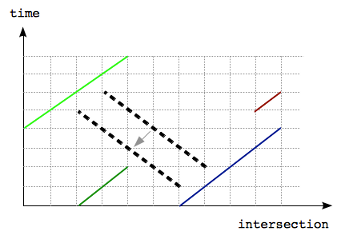
\includegraphics[width=0.8\textwidth]{figgcj2013a_1.png}
				\caption{相距1单位}
			\end{figure}
			
			不过也有特殊情况,这种情况要求我们也考虑与$a_i$的端点横纵坐标都差1的点。如图:
			
			\begin{figure}[ht]
				\centering
				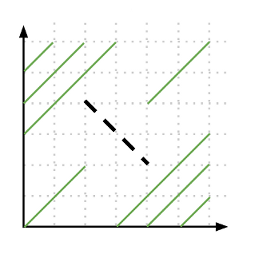
\includegraphics[width=0.6\textwidth]{figgcj2013a_2.png}
				\caption{相距2单位}
			\end{figure}
			
			接下来,枚举这些“必经点”,计算如果线段$l$经过它最多能延伸多长。枚举$a_i$,我们先求直线$l$与它最近的一个(或两个,在两个方向上)的交点在哪,再据此求出其附近最近的一个$l$上的整点。但因为横坐标是循环的,所以略微繁琐。首先求出直线$l$与它任意一个交点的纵坐标$t$(不必最近,也不必为整数),这可以直接解方程得到。注意到所有交点的纵坐标都可以表示为$t+\frac{1}{2}kN$($k$为整数)。接下来确定有用的$k$的范围,记$a_i$起点和终点的纵坐标分别为$T_i$和$R_i$,$\frac{T_i-p}{N} \leq k \leq \frac{R_i-p}{N}$。$k$最多有两种取值,枚举$k$,算出对应交点,再算出最近的整点,更新对$l$的限制,最后取最紧的限制即可。
		
		\myparagraph{时空复杂度}
		
			枚举$a_i$确定必经点,再枚举$a_i$确定$l$最多能延伸多长,其中的每次计算虽然情况很多,但都是线性的。总时间$O(C^2)$,总空间$O(C)$。
	
	\section{CodeJam 2014 Finals C - Symmetric Trees}
	
		\myparagraph{题目大意}
	
			给一棵$N$个节点的树($N \leq 10000$),每个节点有一个颜色(颜色最多26种),现在问它是不是对称的。对称的定义是,能把这棵树放在一个平面上,$x=0$为对称轴,若在$(x,y)$处有一点$v$,那么在$(-x,y)$处就一定有一个相同颜色的点$v'$(如果$x=0$则它们为同一点),并且对于所有边$(u,v)$,$u'$和$v'$间也一定有边。共$T$组数据,$T \leq 100$。
	
		\myparagraph{算法讨论}
		
			分两种情况。如图(图片可能在下一页):
			
			\begin{figure}[ht]
				\centering
				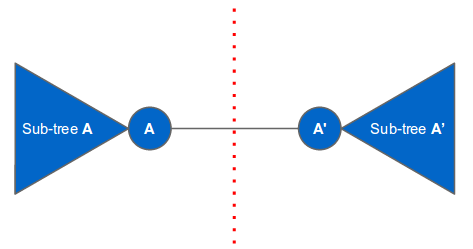
\includegraphics[width=0.8\textwidth]{figgcj2014c_1.png}
				\caption{情况1}
			\end{figure}
			
			\begin{figure}[ht]
				\centering
				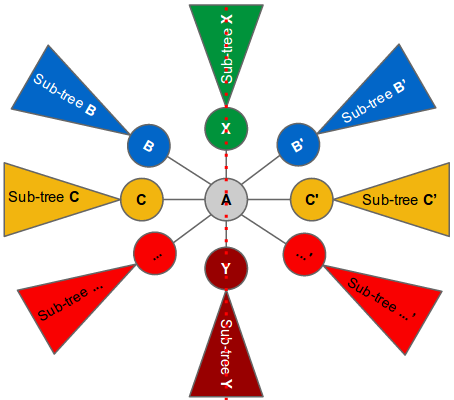
\includegraphics[width=0.8\textwidth]{figgcj2014c_2.png}
				\caption{情况2}
			\end{figure}
		
			即:
		
			\begin{enumerate}
				\item 如果对称轴上没有点,那么树一定能分成两个互相同构的子树。
				\item 否则对称轴上有若干点。任取其中一点,考虑所有以它为根的子树,分为两种。一是图中的$(B,B')$、$(C,C')$等,成对出现,每对相互同构;二是图中的$X$和$Y$,它们本身就是对称的,而且最多只能有两个。
			\end{enumerate}
			
			为了计算两棵子树是否同构以及每棵子树本身是否对称,枚举所有$2N-2$棵子树,计算它的哈希值。为了对树做哈希,我们可以把树看作一个字符串,对其做先序或后序遍历,并用特殊字符标志其中每棵子树的范围,这样即可使用字符串哈希的方法哈希。为了保证以一个节点的子节点为根的子树之间是无序的,需先对这些子树按其哈希值大小排序再进行遍历。当然,为了保证线性时间,要使用记忆化,即对于每个节点,用以其子节点为根的每棵子树的哈希值计算出以该点为根子树的哈希值,而不是每次都重新遍历。CodeJam数据较强,没有依据地随便哈希是不能得出正确答案的。
			
			为了判断一棵子树本身是否对称,将其下(以这棵子树的根的子节点为根的,下同)的互相同构的子树配对,如果所有子树都能配对或者剩下的最多一棵子树本身也是对称的,那么它就是对称的。配对在上文所述排序后扫描即可实现。
			
			最后,如果是第一种情况,直接判断是否存在一条边两侧的的子树哈希值是否相同即可;否则枚举一个点,以它为根,将其下子树按哈希值排序后配对,并检验未配对的子树的对称性即可得出答案。
		
		\myparagraph{时空复杂度}
	
			预处理所有子树的哈希及其本身的对称性时,需枚举所有$2N-2$棵子树,并对其下所有子树按哈希值排序,考虑上数据组数,总时间复杂度$O(TN\log_2N)$。总空间复杂度$O(N)$。
	
	\section{CodeJam 2014 Finals D - Paradox Sort}
	
		\myparagraph{题目大意}
		
			有$n$个糖果($n \leq 100$),对于每对糖果,Vlad都更喜欢其中的一个,但是它的偏好不一定满足偏序关系。你要按一定顺序依次给他$n$个糖果,每时每刻Vlad只拿着一颗。每次如果相比手上的,他更喜欢新的,它就扔掉手上的拿新的,否则不拿新的。你要设计一个这样的顺序,使他最后拿着的糖果编号为$A$,如果有多解输出字典序最小的顺序。有$T$组数据,$T \leq 100$。
		
		\myparagraph{算法讨论}
		
			首先我们要能判断是否有解。对于每一对糖果$(x,y)$,如果Vlad更喜欢$x$,就连一条$x$到$y$的边,否则连一条$y$到$x$的边。以$A$为根,DFS遍历整个图,如果所有点(糖果)都被遍历到了,那么有解,否则无解。
			
			\begin{proof}\mbox{}\\
			
				如果所有点都被遍历到了,可以构造一棵DFS树,此树的后序遍历就是一个合法解。原因如下:记当前遍历到$y$点,手上拿着的糖果是$x$点,$x$肯定被遍历过。如果$x$是已经遍历过的点中深度最浅的,按照后序遍历的特点,$y$最浅的可能深度也只能比$x$的深度小1,而且此时必然有边$y \to x$,Vlad会扔掉$x$拿$y$,手上拿的仍然是深度最浅的一个。而一开始只有一个点被遍历过时,$x$必然是最浅的一个。所以最后Vlad拿着的一定是根节点对应的糖果。
				
				如果有点没被遍历到,假设该点为$p$。对于能遍历到的部分任意点$q$,都有边$q \to p$。如果给Vlad遍历过的点,再给$p$,他就一定会拿$p$;反之先给$p$,它就永远拿不到遍历过的点,包括$A$。
				
			\end{proof}
			
			下一步我们要求字典序最小。因为是字典序,如果前面的糖果编号大了,后面的糖果编号再小也没用,所以我们使用贪心。一个糖果一个糖果地构造答案序列。假设当前构造到第$i$个,从小到大尝试第$i$个是什么,如果加上此糖果就有解了,就用此糖果,继续做第$i+1$个,否则继续尝试更大编号的糖果。
			
			不过因为已经选了$i$个糖果了,判断是否有解的方法较上面更复杂。记给完这$i$颗糖果,Vlad手上拿着的是糖果$B$。分两种情况讨论。
			
			\begin{enumerate}
				\item 如果$A$在这$i$颗糖果中,假设$A \not= B$,显然无解。否则仅对于所有没给过的糖果$j$都有边$i \to j$的情况才有解。
				\item 否则,仍以$A$为根遍历,但不访问$B$,最后再把$B$和所有满足有边$B \to x$的点$x$加入DFS树。此树的后序遍历是合法解,理由类似上面。
			\end{enumerate}
			
		\myparagraph{时空复杂度}
		
			首先要枚举$i$,再$O(n)$枚举第$i$颗糖是什么,再$O(n)$遍历判断是否有解,考虑上数据组数$T$,时间复杂度$O(n^3T)$。空间复杂度为存图的空间复杂度,为$O(n^2)$。
	
	\section{CodeJam 2014 Finals E - Allergy Testing}
	
		\myparagraph{题目大意}
	
			Kelly对$N$种食物中的一种过敏,她要做试验找出到底对哪种过敏。每次她可以选一部分食物吃,等$A$天后如果没有过敏反应,则使她过敏的食物不在这一部分里,否则在,而且她还要继续等$B-A$天等反应消去才能进一步实验。为了实验的严谨性,必须等上一次试验结束之后(等了$A$天或$B$天)才能做下一次试验。给定$N$、$A$、$B$,问最少要花多少天Kelly才能确定对哪种食物过敏。$1 \leq N \leq 10^{15}, 1 \leq A \leq B \leq 10^{12}$。
	
		\myparagraph{算法讨论}
		
			用DP解决。一个显然的方法是用还需要试验的食物种数作状态,但这样最快只能优化到$O(N)$。按另一种思路,可以以剩余天数作状态,设$f[i]$表示用$i$天最多能试验多少食物,假设求得了$f$,即可二分答案出解。考虑转移方程:当前有$i$天时间,假设要先吃$x$种,还剩$y=f[i]-x$种。如果过敏了,就要等$B$天,然后要在$i-B$天内在这$x$种中确定过敏原;否则就要等$A$天,然后在$i-A$天内在$y$种中确定过敏原。为了使$x$和$y$尽量大,$x=f[i-B], y=f[i-A]$。所以转移方程为
			
			$$f[i]=x+y=f[i-A]+f[i-B]$$
			
			还要考虑边界状态。显然$f[i]=1$当且仅当$i<A$。另外如果$x=1$,吃完后即使过敏也不用等它消退,只用等$A$天。但如果$i-A \leq B \Leftrightarrow i-B \leq A$,那么$x=f[i-B]>1$更优,所以$x=1$只存在于$i-B<A$时,不妨仍把它写成$x=f[i-B]=1$,两者等价。所以总方程为
			
			$$f[i]=\left\{\begin{array}{ll}
				f[i-A]+f[i-B] & i \geq A \\
				1 & i<A \mbox{(此处允许负数)}
			\end{array}\right.$$
			
			这样的算法仍不能被接受,要继续优化。假设二分答案时我们二分到了$D$天,把DP的转移树画出来,根为$f[D]$,对于每个节点$f[i]$,$f[i-A]$和$f[i-B]$分别是它的两个子节点。$f[i]=1$的点为叶节点,$i<A$。$f[D]$等于整棵树上叶节点的个数。每个叶节点对应一条从根出发到它的路径,路径上的每条边要么是$-A$转移要么是$-B$转移。所以我们可以枚举总共有$i$个$-A$转移,$j$个$-B$转移,则
			
			$$f[N]=\sum_{D-A<iA+jB\leq D}\binom{i+j}{j}$$
			
			可以用树高估计数的规模,因为$B>A$,所以$f[N]>2^j \Rightarrow j<\log_2f[N]$,$j$最多只有60,所以可以枚举$j$。
			
			$$\begin{aligned}
				f[N]&=\sum_{j=1}^{60}\sum_{i=\lfloor \frac{D-jB-B}{A} \rfloor+1}^{\lfloor \frac{D-jB}{A} \rfloor} \binom{i+j}{j} \\
				    &=\sum_{j=1}^{60}(\binom{\lfloor \frac{D-jB}{A} \rfloor+j+1}{j+1}-\binom{\lfloor \frac{D-jB-B}{A} \rfloor+1+j}{j+1})
			\end{aligned}$$
			
			二分答案后直接计算此式就能出解。为了避免算术溢出,可以使用浮点数近似计算,也可以写高精度。
		
		\myparagraph{时空复杂度}
		
			二分答案$O(\log_2N)$,枚举$j$需$O(\log_2{f[N]})$,计算组合数需$O(j)=O(\log_2{f[N]})$。$\log_2{f[N]}<\log_2N$,所以$O(\log_2{f[N]})=O(\log_2N)$。总时间复杂度$O(\log_2^3{N})$。空间复杂度$O(1)$。
	
	\section{CodeJam 2014 Finals F - ARAM}
	
		\myparagraph{题目大意}
		
			游戏中有$N$个英雄($N \leq 1000$),你用其中每个玩一局都有一个相应的胜率$P_i$。现在你要玩$10^{100}$局,每局开始前要随机抽一个英雄用,如果对抽到的英雄不满意可以重抽,重抽依然是随机的。每次重抽要用一块钱,只要有钱就可以重抽任意次。最初有$R$块钱,每次玩完一局,不管输赢都能挣$1/G$块钱($R,G \leq 20$)。求期望赢的局数占总局数$10^{100}$的比例的最大值。有$T$组数据。
		
		\myparagraph{算法讨论}
		
			由于$10^{100}$很大,可以当作无限大考虑,这样每次决定是否重抽仅与当前剩余的钱数和抽到了什么英雄有关。显然剩余钱数相同时,使我们决定要重抽的英雄的胜率一定比使我们决定不重抽的英雄的要低,所以对于特定的剩余钱数,肯定是英雄胜率小于某临界值时就重抽,否则不重抽。
			
			我们要求的是赢的局数占总局数的比例,不便于处理,可以通过二分答案去除总局数的影响:设二分到的答案为$K$,再设$f[i]$表示目前剩余$i$块钱时,一直玩直到钱数大于$i$期间,胜利数相比二分出的答案多了(或少了)多少。$f[i]$表示的是总的胜利数,不用除总局数。
			
			$0 \leq i < 1$时,不能重抽,所以
			
			$$f[i]=\frac{1}{N}\sum_{j=1}^N(P_j-K)$$
			
			$1 \leq i < R$时,记如果抽到了胜率前$X_i$小的英雄要重抽,
			
			$$f[i]=\min_{X_i} \frac{X_i}{N}\sum_{j=0}^G f[i-1+\frac{j}{G}] + \frac{1}{N}\sum_{j=X_i+1}^N(P_j-K)$$
			
			$i=R$时,稍修改一下定义,$f[R]$是一直玩直到钱数再次等于$R$期间胜利数相比二分出的答案的盈余或亏损。
			
			$$f[R]=\min_{X_i} \frac{X_i}{N}\sum_{j=0}^{G-1} f[i-1+\frac{j}{G}] + \frac{1}{N}\sum_{j=X_i+1}^N(P_j-K)$$
			
			$f[R]>0$时,说明$K$小了;$f[R]<0$时,说明$K$大了。为什么?虽然这样算结束时还有$R$块钱,答案理应更大些,但是用完这$R$块钱能多出的胜率在$10^{100}$局面前是微不足道的,所以可以用$f[R]$判断二分的调整方向,这样此题得解。
		
		\myparagraph{时空复杂度}
		
			二分与精度有关,简记为$O(log)$。每次二分要做状态$O(RG)$,每次转移$O(N)$的DP。考虑$T$组数据,总时间复杂度$O(T \cdot log \cdot RG)$。总空间复杂度$O(RG+N)$。
	
	\section{USACO 2007 Dec gold 3 - Best Cow Line, Gold}
	
		\myparagraph{题目大意}
		
			有一个长度为$n$的字符串$s$($n \leq 30000$),还有一个初始为空串的字符串$t$。每次可以从$s$头部或尾部删除一个字符,并将其加入到$t$尾部,直到$s$为空。求字典序最小的$t$。
		
		\myparagraph{算法讨论}
		
			假设当前$s$的首尾字符不同,显然应该删去较小的那个。拓展到一般情况,比较此字符串及其逆序串的字典序,应当优先删除字典序小的那个方向。可以把原串及其逆序串连接起来,建一个后缀数组,这样每次就可以在常数时间比较两个字符串的大小了。
		
		\myparagraph{时空复杂度}
		
			$O(n\log_2n)$建后缀数组,随后$O(n)$扫描比较。总时间$O(n\log_2n)$。总空间$O(n)$。
	
	\section{USACO 2012 Dec gold 2 - First!}
		
		\myparagraph{题目大意}
		
			有$n$个字符串,总长$l$($1 \leq n \leq 30000, 1 \leq l \leq 300000$)。字符集$\Sigma$为小写字母,你可以通过改变$\Sigma$中字符的顺序改变字符串的字典序。问这些字符串中有多少个可以通过这种方法变成字典序最小的。
		
		\myparagraph{算法讨论}
		
			假设字符串$s_1$字典序比$s_2$小,它们在第$i$格字符前都相同,那么$s_1[i]<s_2[i]$,$i$后的字符大小关系都没有影响。扫描每个字符串$s_x$,它和每个其它的字符串$s_y$都可以形成一个字符的大小关系要求,比如'b'$<$'a'。用这种关系建图,如果图中有环则不可行,用Tarjan等方法即可在$O(|\Sigma|)$时间内判断,用SPFA等$O(|\Sigma|^2)$的方法也能通过,因为这里不是时间瓶颈。对所有的字符串建一棵TRIE树即可在枚举$x$时快速找出字符大小关系的要求,即遍历到TRIE的每个点时扫描其兄弟,把大小关系加入图中,在退出该节点时还原。每次扫描的时间也是$O(|\Sigma|)$。
		
		\myparagraph{时空复杂度}
		
			建TRIE时间$O(l)$,遍历并得出大小关系时间$O(l|\Sigma|)$,对每个字符串判断是否可能$O(n|\Sigma|)$,总时间复杂度$O(l|\Sigma|)$。总空间使用决定于TRIE的使用,直接存储的空间复杂度为$O(l|\Sigma|)$,使用“左儿子右兄弟”存储可使空间复杂度降为$O(l)$。
	
\end{document}